\documentclass{article}

\usepackage{amsmath}
\usepackage{amssymb}
\usepackage{amsthm}
\usepackage{enumerate}
\usepackage{relsize}
\usepackage{algorithm}
\usepackage{algpseudocode}
\usepackage{parskip}
\usepackage{graphicx}
\usepackage{cite}
\graphicspath{{images/}}

\usepackage[
  top    = 2.75cm,
  bottom = 3.00cm,
  left   = 2.50cm,
  right  = 2.50cm
]{geometry}

\algnewcommand\algorithmicinput{\textbf{Input:}}
\algnewcommand\algorithmicoutput{\textbf{Output:}}
\algnewcommand\algorithmicsideeffect{\textbf{Side Effect:}}
\algnewcommand\Input{\item[\algorithmicinput]}
\algnewcommand\Output{\item[\algorithmicoutput]}
\algnewcommand\SideEffect{\item[\algorithmicsideeffect]}
\algnewcommand{\IIf}[1]{\State\algorithmicif\ #1\ \algorithmicthen}
\algnewcommand{\IIEf}[2]{\State\algorithmicif\ #1\ \algorithmicthen\ #2\ \algorithmicelse}
\newcommand{\compatible}{\smile}
\newcommand{\leafset}{\Lambda}

\title{A Faster Construction of Frequency Difference Consensus Trees\\CG4001 Interim Report}
\author{Varun Gupta\\A0147924X}

\newtheorem{incompatibility}{Lemma}
\newtheorem{freqdiffruntimecomponents}[incompatibility]{Corollary}
\newtheorem{lca}[incompatibility]{Lemma}
\newtheorem{linearrmq}[incompatibility]{Lemma}
\newtheorem{cfd}[incompatibility]{Lemma}
\newtheorem{rmqinc}[incompatibility]{Lemma}
\newtheorem{rmqstructure}[incompatibility]{Theorem}
\newtheorem{assocnode}[incompatibility]{Lemma}
\newtheorem{labelclusterscorrectness}[incompatibility]{Lemma}
\newtheorem{labelclustersidbounds}[incompatibility]{Lemma}
\newtheorem{labelclustersruntime}[incompatibility]{Lemma}
\newtheorem{weightingruntime}[incompatibility]{Lemma}
\newtheorem{filterclusterssubsetcompatible}[incompatibility]{Lemma}
\newtheorem{incompatibilityrootsofsubtrees}[incompatibility]{Lemma}
\newtheorem{incompatibilityrecursive}[incompatibility]{Lemma}
\newtheorem{computerootsofsubtreescorrectness}[incompatibility]{Lemma}
\newtheorem{computerootsofsubtreesruntime}[incompatibility]{Lemma}
\newtheorem{filterclustersruntime}[incompatibility]{Lemma}
\newtheorem{freqdiffruntime}[incompatibility]{Theorem}

% TODO:
% Improvements:
% 1. What have I contributed?
% 2. Captions

\begin{document}
    \maketitle

    \begin{abstract}
        This report presents a new deterministic algorithm for constructing a frequency difference consensus tree. Given $k$ phylogenetic trees with identical leaf label sets of size $n$, this algorithm constructs the frequency difference tree in $O(kn\,log\,n)$ time, bettering the previously best known time of $O(kn\,log^2n)$.
    \end{abstract}

    \section{Introduction}
    \label{sec:introduction}

    A \textit{taxon} (pl. taxa) is a group of organisms that taxonomists classify as a single unit, such as \textit{homo sapiens}. These come together to give a \textit{rooted phylogenetic tree}, which presents the evolutionary relationships between various taxa in a hierarchical manner. Here, each node represents the common ancestor of a subgroup of taxa and children of nodes split each group into smaller ones. A subgroup of taxa that are descendants of some common ancestor is called a \textit{clade}, i.e. a clade is the leaf set of any node in a phylogenetic tree.

    We often obtain multiple phylogenetic trees from biological datasets. For example, these may be produced from different datasets or from a single dataset using techniques like maximum parsimony that yield a number of candidate trees \cite{bryant1997hunting}. This motivates the concept of a \textit{consensus tree}, which reconciles many phylogenetic trees by summarising the branching information contained in each into a single tree. Consensus trees are also useful in determining which clades have strong suppport within the input trees \cite{felsenstein2004inferring}.

    A variety of techniques of constructing a consensus tree from a set of phylogenetic trees have been developed over the last half century, starting with the Adams consensus tree \cite{adams1972consensus} in 1972. There is strong motivation for the development of different types of consensus trees since they each have their own benefits and drawbacks. Some of these techniques are summarised in \S 6.2 of \cite{bryant1997hunting} and a comparative analysis can be found in \cite{bryant2003classification}. We illustrate with some examples. The \textit{strict consensus tree} \cite{sokal1981taxonomic} only keeps those clades that occur in each of the input trees. While easily constructed and interpreted, it can discard a lot of potentially important information if there is a lot of disagreement between the various trees. The \textit{majority rule consensus tree} \cite{margush1981consensusn} is a generalisation of the previous, allowing all clades that occur in a majority of the trees. Holder et al. \cite{holder2008justification} showed that these trees are optimal given a certain context.

    This article studies a specific type of consensus tree, known as the \textit{frequency difference consensus tree} \cite{goloboff2003improvements}. The \textit{frequency difference consensus tree} (abbreviated henceforth as FDCT) further generalises the \textit{majority rule consensus tree}, keeping every clade that occurs in more trees than the most frequent clade that contradicts it (the concept of contradiction is formalized in Subsection~\ref{subsec:def}). The FDCT is motivated by a desire to design an effective criterion for determining which clades are strongly supported within a set of trees. As set out in \cite{goloboff2003improvements}, a shortcoming of the majority rule consensus tree is that it would include a clade that is supported by 60\% of a set of trees and contradicted by 40\% of them. Conversely, a clade supported by 40\% of the trees but not contradicted by any of them would not appear in the consensus tree. A possible resolution to this is to define strongly supported clades as those with greater frequency than all clades incompatible with them. These are called frequency difference clades and all of these are included in the FDCT.

    Dong et al. \cite{dong2010majority} provided a comparison of the FDCT and a few other types of consensus trees. Barrett et al. \cite{barrett2013plastid} employed the idea of using frequency difference as a measure of clade support while analysing angiosperm phylogeny and commented ``[the] frequency difference metric ... is particularly useful for assessing support when it is not overwhelmingly in favour of one particular topology, and should be especially useful in phylogenomic analyses in general, where hundreds or thousands of characters may contribute to branch support''. Steel and Velasco \cite{steel2014axiomatic} investigated a generalisation of the FDCT to \textit{supertrees}, i.e. consensus trees built from input trees that do not necessarily have the same leaf sets. They show that, unlike some other popular techniques, the FDCT definition easily generalises to a viable supertree definition and conclude that the FDCT is ``worthy of more widespread usage and serious study''. Given that the FDCT has been utilised in various studies over the years \cite{garcia2014testing,barrett2013plastid,molineri2010cladistic,molineri2013phylogeny,molineri2015phylogeny,lindqvist2006molecular} and keeping in mind the favourable opinions above, we set out to improve upon the best known deterministic algorithm for constructing the FDCT of a set of trees.

    \subsection{Definitions and Notation}
    \label{subsec:def}

    We define a rooted phylogenetic tree to be a rooted, leaf-labelled tree where every internal node has 2 or more children and every leaf has a different label. Henceforth, we will simply refer to these as trees. Let $T$ be some tree. The set of nodes of $T$ is denoted by $V(T)$. For any node $u \in V(T)$, the \textit{parent} of $u$ (if it exists) is represented by $parent^T(u)$ and the set of its \textit{children} is represented by $children^T(u)$. The \textit{depth} of $u$, denoted by $depth^T(u)$ is the number of nodes that are its proper ancestors. A node that is \textit{shallower} than another has a smaller depth value. Non-empty subsets of $\leafset^T$ are called \textit{clusters} (we use the term clusters instead of clades for consistency with recent literature). Clusters with cardinality $1$ or $|\leafset^T|$ are \textit{trivial clusters}. For any node $u \in V(T)$, $T[u]$ is the subtree of $T$ rooted at $u$ and $\leafset^T(u)$ is the leafset of $T[u]$, called the cluster \textit{associated} with $u$. For example, in Figure~\ref{fig:freqdiff}, the node labelled by $2$ in $T_1$ has the cluster $\{a, b\}$ associated with it. The subtree rooted at this node is the tree consisting of the node itself, and the two leafs that are its children. The \textit{cluster collection} of $T$, $\mathcal{C}(T)$ is the set $\bigcup_{u \in V(T)} {\leafset(u)}$, i.e. a set containing all the clusters in $T$. For example, the cluster collection of $T_1$ in Figure~\ref{fig:freqdiff} is $\{\{a\}, \{b\}, \{c\}, \{d\}, \{e\}, \{a, b\}, \{c, d, e\}, \{a, b, c, d, e\}\}$. Any cluster $C \subseteq \leafset(T)$ \textit{occurs} in $T$ iff $C \in \mathcal{C(T)}$. Also define, for any tree $T$, for any set of nodes $U \subseteq V(T)$, $lca^T(U)$ to be the least common ancestor of $U$ in $T$.

    Any two clusters $C_1, C_2 \subseteq \leafset(T)$ are said to be \textit{compatible}, denoted as $C_1 \compatible C_2$, iff $C_1 \subseteq C_2$ or $C_2 \subseteq C_1$ or $C_1 \cap C_2 = \emptyset$. If $C_1$ and $C_2$ satisfy none of the preceding properties, then they are said to be \textit{incompatible} (referred to as \textit{contradiction} in Section~\ref{sec:introduction}), denoted as $C_1 \not\compatible C_2$. Similarly, given trees $T_1$ and $T_2$ with identical leaf sets, and nodes $u \in V(T_1)$, $v \in V(T_2)$, we say $u$ is compatible with $v$ if the clusters associated with $u$ and $v$ are compatible. For example (referring to Figure~\ref{fig:freqdiff}), let $u$ be the node in $T_1$ associated with the cluster $\{a, b\}$, $v$ the node in $T_2$ associated with $\{a, b, c\}$ and $w$ the node in $T_2$ associated with $\{b, c\}$. Then $u$ and $v$ are compatible since $\leafset^{T_1}(u) \subseteq \leafset^{T_2}(v)$. However, $u$ is incompatible with $w$ since they share $b$ but neither leafset is a subset of the other. We now extend the notion of compatibility to trees. A cluster $C \subseteq \leafset(T)$ is \textit{compatible} with $T$ iff for every $C_1 \in \mathcal{C}(T)$, $C \compatible C_1$. Further, two trees $T_1$ and $T_2$ with identical leafsets are \textit{compatible} iff for every $C \in \mathcal{C}(T_1)$, $C \compatible T_2$, i.e. if every cluster in $T_1$ is compatible with $T_2$. Observe that this also means that every cluster in $T_2$ is compatible with $T_1$. Thus in Figure~\ref{fig:freqdiff}, $T_1$ is incompatible with $T_2$ since the former contains the cluster $\{a, b\}$ which is incompatible with $\{b, c\}$, contained in the latter tree (in fact, it can be checked that all the trees in this figure are incompatible).

    \begin{figure}[h]
        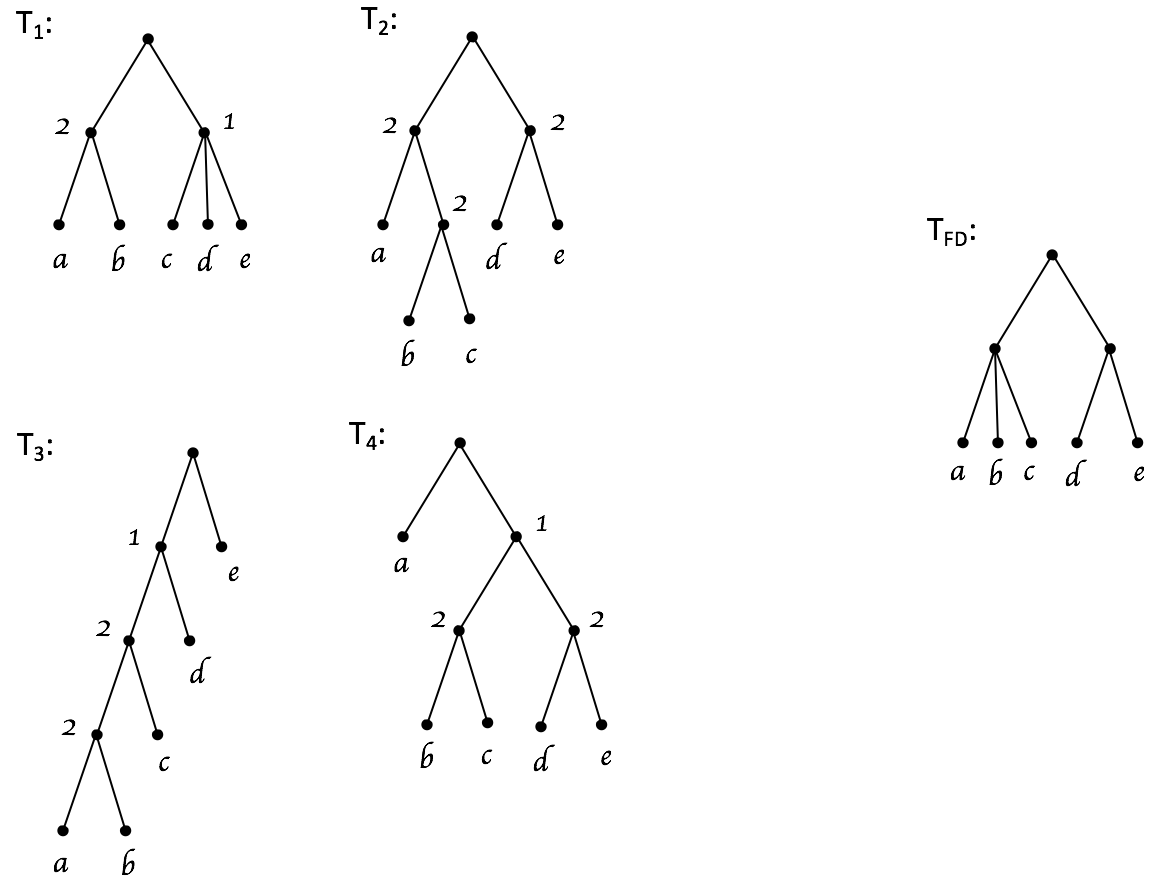
\includegraphics[scale=0.5]{freqdiff}
        \centering
        \caption{$T_{FD}$ is the FDCT of $\{T_1, T_2, T_3, T_4\}$}
        \label{fig:freqdiff}
    \end{figure}

    A \textit{frequency difference consensus tree} is defined as follows. Let $\mathcal{S}$ be a set of $k$ trees with identical leaf labels, i.e. $\mathcal{S} = \{T_1, T_2, ..., T_k\}$, where $\leafset(T_1) = \leafset(T_2) = ... = \leafset(T_k) = L$. For any cluster $C \subseteq L$, let $K_C = \{T : T \in \mathcal{S} \text{ and } C \in \mathcal{C}(T)\}$ be the set of trees in $\mathcal{S}$ which $C$ occurs in. Then $T_{FD}$ is the FDCT of $\mathcal{S}$, where $\mathcal{C}(T_{FD}) = \{C : C \subseteq L \text{ and } |K_C| > max(\{|K_{C_1}| : C_1 \subseteq L \text{ and } C \not\compatible C_1\})\}$. Thus $T_{FD}$ contains all clusters that occur more frequently than any cluster that they are incompatible with. By Proposition $3$ in \cite{steel2014axiomatic}, this tree always exists and is unique for a given $\mathcal{S}$. Figure~\ref{fig:freqdiff} gives an example. In this, $|K_{\{a, b\}}| = 2 \leq |K_{\{b, c\}}| = 2$ and $\{a, b\} \not\compatible \{b, c\}$, hence $\{a, b\}$ is not in the final consensus tree. However $\{a, b, c\}$ and $\{d, e\}$ have frequencies greater than any cluster incompatible with them, hence they both exist in the consensus tree. Note that frequencies are not shown for the trivial clusters.

    Finally, for any tree $T$, for any nodes $v, w \in V(T)$, where $w$ is an ancestor of $v$, define $pathInc^{T}(v, w)$ to be the set of nodes that are ancestors of $v$ and descendants of $w$ and $path^{T}(v, w)$ to be the set of nodes that are ancestors of $v$ and \textit{proper} descendants of $w$. That is, $pathInc^{T}(v, w)$ contains all nodes on the path from $v$ to $w$, while $path^{T}(v, w)$ is the same set, excluding $w$. Notice that $path^{T}(v, w) = \emptyset$ when $v = w$.

    For each of the definitions above where the tree is specified in the superscript, this superscript is omitted if the tree being referred to is clear from context. For example, $children^T(u)$ would be written as $children(u)$. This will also be applied to any notation developed in the remainder of this text.

    Henceforth, $\mathcal{S}$ is taken to be the input set of trees with identical leaf labels. This set of leaf labels is denoted by $L$. Let $|\mathcal{S}| = k$ and $|L| = n$.

    \subsection{Previous Work}
    An implementation of the FDCT can be found in the free software package TNT \cite{goloboff2008tnt}; however the algorithm used within is unavailable and so its complexity is not known. Jansson et al. \cite{jansson2018algorithms} gave a deterministic $min\{O(kn^2), O(kn(k + log^2 n))\}$ algorithm for constructing the FDCT, implemented in the open source FACT package \cite{jansson2016improved}. Gawrychowski et al. \cite{gawrychowski2017faster} improved upon this to give a deterministic $O(kn\,log^2n)$ algorithm (not yet implemented).

    \subsection{Organisation of the Article and New Results}
    Section~\ref{sec:preliminaries} contains some results from previous works that are utilised later. Section~\ref{sec:rmqstructure} shows how an efficient range minimum/maximum query structure can be built on trees. Section~\ref{sec:freqdiffconstruction} presents a new deterministic algorithm for constructing the FDCT that runs in $O(kn\,log\,n)$ time.

    \section{Preliminaries}
    \label{sec:preliminaries}

    \subsection{The \textit{lca} operation}

    We restate the following lemma outlining the \textit{lca} operation from \cite{bender2000lca}:
    \newline

    \begin{lca}
        \label{lem:lca}

        Given any tree $T$ and nodes $u, v \in V(T)$, $lca(u, v)$ is the deepest node in $T$ that is an ancestor of $u$ and $v$. $lca(u, v)$ can be answered in constant time, given $O(n)$ preprocessing time, where $n = |V(T)|$.
    \end{lca}

    \subsection{The linear RMQ data structure}

    We restate the following lemma outlining the \textit{linear RMQ data structure} from \cite{bender2000lca}:
    \newline

    \begin{linearrmq}
        \label{lem:linearrmq}

        Given an array $A$ of numbers of length $n$, and indices $i, j$, the query $rmqLin^A(i, j) = max_{i \leq k \leq j}A[k]$ can be answered in constant time, given $O(n)$ preprocessing time.
    \end{linearrmq}

    \subsection{Centroid Path Decomposition}

    The \textit{centroid path decomposition technique} of \cite{cole2000n} is used to decompose a tree $T$ into a path from the root to some leaf and a set of disjoint subtrees. A \textit{centroid path} in $T$ is the path formed by starting at the root and at each point following the child with the largest leaf set. The centroid path is denoted by $\pi = \langle p_{\alpha}, p_{\alpha - 1}, ..., p_1 \rangle$, where $p_{\alpha}$ is the root of $T$ and $p_1$ is a leaf. Removing the path $\pi$ from $T$ results in a set of disjoint subtrees of $T$, where the root of each such subtree is a child of some node in $\pi$. These trees are called the \textit{side trees} of $\pi$, denoted by $\sigma(\pi)$. Also let $\sigma(p_i)$ be the set of side trees whose roots are children of $p_i$, called the side trees \textit{associated} with $p_i$. Figure~\ref{fig:centroid} demonstrates this decomposition. Here, the bold path from the root to leaf is the centroid path. When the dashed edges and the nodes contained in the centroid path are removed from the tree, the side trees remain. In particular, it can be seen that there are two side trees associated with the root, one containing three nodes and the other containing just a single leaf.

    \begin{figure}[h]
        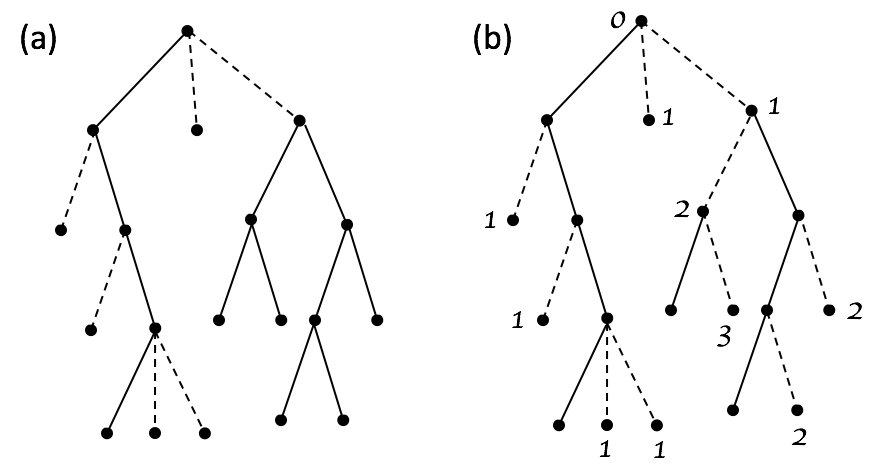
\includegraphics[scale=0.5]{centroid}
        \centering
        \caption{Example of centroid path decomposition}
        \label{fig:centroid}
    \end{figure}

    \subsection{The \textit{delete} operation}
    \label{subsec:delete}
    As described in \cite{jansson2018algorithms}, the \textit{delete} operation deletes a cluster from a tree. To do so, we specify some internal node $u$ in a tree $T$, such that we wish $\leafset(u)$ to be deleted. Then the \textit{delete} operation makes $parent(u)$ the parent of all nodes in $children(u)$ and removes $u$, along with any associated edges from $T$. This has the effect of removing only $\leafset(u)$ from $T$, without affecting any other cluster. For example, in Figure~\ref{fig:freqdiff}, if we perform a delete operation on $T_2$, on the node associated with the cluster $\{b, c\}$, the resulting tree is identical to $T_{FD}$.

    \subsection{Characterising incompatibility}
    We restate Lemma 6 of \cite{jansson2018algorithms} here since it is crucial in the development of an algorithm discussed below:
    \newline

    \begin{incompatibility}
        \label{lem:incompatibility}

        Given a tree $T$ and a cluster $C \subseteq \leafset(T)$, let $l_C = lca^T(C)$. Then for any $u \in V(T)$, $C \not\compatible \leafset(u)$ iff $u$ lies on the path between $l_C$ and some $x \in C$ and $\leafset(u) \not\subseteq C$.
    \end{incompatibility}

    \subsection{The \texttt{Merge\_Trees} algorithm}
    \label{subsec:mergetrees}

    As described in \cite{jansson2016improved}, the \texttt{Merge\_Trees} algorithm takes as input trees $T_1$ and $T_2$, where $\leafset(T_1) = \leafset(T_2) = L$ and $T_1$ is compatible with $T_2$. It returns a tree $T$ with $\leafset(T) = L$ and $\mathcal{C}(T) = \mathcal{C}(T_1) \cup \mathcal{C}(T_2)$ in $O(|L|)$ time.

    \subsection{The \texttt{Frequency\_Difference} algorithm}
    The algorithm \texttt{Frequency\_Difference} is laid out in \cite{jansson2018algorithms}. Before describing it, we first define the weight of a node $u$ to be the number of trees in $\mathcal{S}$ that the cluster associated with $u$ occurs in. Formally, for any tree $T \in \mathcal{S}$ and any node $u \in V(T)$, let $C = \leafset(u)$, then the weight of $u = \Omega(u) = |K_C|$ and $\Omega(C) = \Omega(u)$. The procedure \texttt{Filter\_Clusters} is defined to take in trees $T_A$ and $T_B$, with $\leafset(T_A) = \leafset(T_B) = L$ and the values of $\Omega(u)$ for all $u \in V(T_A) \cup V(T_B)$. It returns a tree $T$ which contains all clusters $C$ in $T_A$ for which $\Omega(C) > $ weight of all clusters in $T_B$ that it is incompatible with. Formally, \texttt{Filter\_Clusters}$(T_A, T_B) = T$ where $\mathcal{C}(T) = \{C : C \in \mathcal{C}(T_A) \text{ and } \Omega(C) > max(\{\Omega(C_1) : C_1 \in \mathcal{C}(T_B) \text{ and } C_1 \not\compatible C\})\}$ and $\leafset(T) = L$. For example, referring to Figure~\ref{fig:freqdiff}, \texttt{Filter\_Clusters}$(T_2, T_1) = T_{FD}$. Notice that there are three non-trivial clusters in $T_2$: $\{a, b, c\}, \{b, c\}$ and $\{d, e\}$. All of these have weight $2$. Now the only cluster in $T_1$ incompatible with $\{a, b, c\}$ is $\{c, d, e\}$, but this only has weight $1$ and so $\{a, b, c\}$ is kept. The cluster $\{d, e\}$ is compatible with $T_1$ so it is also kept. However, $\{b, c\}$ is incompatible with $\{a, b\}$ and they both have weight $2$, hence $\{b, c\} \not\in \mathcal{C}($\texttt{Filter\_Clusters}$(T_2, T_1))$.

    The algorithm \texttt{Frequency\_Difference} runs in two parts. First, for any tree $T \in \mathcal{S}$ and any node $u \in V(T)$, it computes $\Omega(u)$ in the \textit{weighting} step. In the second part, it utilises \texttt{Filter\_Clusters} and \texttt{Merge\_Trees} (from Subsection~\ref{subsec:mergetrees}) to compute the FDCT. Theorem 3 of \cite{jansson2018algorithms} gives the following corollary:
    \newline

    \begin{freqdiffruntimecomponents}
        \label{cor:freqdiffruntimecomponents}

        The total runtime of \texttt{Frequency\_Difference} is given by $O(g(n, k) + k \cdot f(n))$ where $g(n, k)$ is the time taken by the weighting step and $f(n)$ is the runtime of \texttt{Filter\_Clusters}.
    \end{freqdiffruntimecomponents}

    Jansson et al. \cite{jansson2018algorithms} gave a $min(\{O(kn^2), O(k^2n)\})$ solution to the weighting step and an $O(n\,log^2n)$ solution to \texttt{Filter\_Clusters}, giving an overall runtime of $min(\{O(kn^2), O(kn(k + log^2n))\})$. Gawrychowski et al. \cite{gawrychowski2017faster} improved the runtime of the weighting step to $O(kn\,log^2n)$, thus reducing the overall runtime to $O(kn\,log^2n)$.

    \section{RMQ (range minimum/maximum query) structure on trees}
    \label{sec:rmqstructure}

    Given a tree $T$ with $\Omega(u)$ defined for each $u \in V(T)$, we build a data structure capable of answering the query, for any nodes $v, w \in V(T)$ where $w$ is a proper ancestor of $v$, $rmq^T(v, w) = max_{u \in path(v, w)}\Omega(u)$ in constant time. Recall that $path(v, w)$ is the set of nodes on the path from $v$ to $w$, excluding $w$.

    The $rmq$ query will be answered in two steps. First, given some nodes $v, w \in V(T)$ we obtain the child of $w$ that is an ancestor of $v$ (represented by $cFD(v, w)$). Second, we build the capability to answer the question, given nodes $v, w \in V(T)$, $rmqInc^T(v, w) = max_{u \in pathInc(v, w)}\Omega(u)$. It is then clear that $rmq(v, w) = rmqInc(v, cFD(v, w))$.

    \subsection{Answering $cFD(v, w)$}

    \begin{cfd}
        \label{lem:cfd}

        Given a tree $T$ and nodes $v, w \in V(T)$ such that $w$ is a proper ancestor of $v$, the query $cFD(v, w) =$ child of $w$ that is an ancestor of $v$ can be answered in constant time, given $O(n\,log\,n)$ preprocessing time.

        \begin{proof}
                The $cFD(v, w)$ query is divided into two parts. First, we check if $v$ is a descendant of the heaviest child of $w$. If so, we are done. If not, we work out which of the other children of $w$ is an ancestor of $v$.

                To answer the first part, we apply Lemma~\ref{lem:lca} to preprocess $T$ for $lca$ queries. Then it is easy to see that, given nodes $r, s \in V(T)$, $s$ is an ancestor of $r$ iff $lca(r, s) = s$, thus we can work out whether $v$ is a descendant of the heaviest child of $w$.

                For the second part, first rearrange the tree such that the heaviest child of each node is its leftmost child and then index the leaves left to right. Take any node $u \in V(T)$. Let $x$ be the leftmost leaf in its side trees and $y$ be the rightmost leaf in its side trees. Then build the array $cFL_u[1\, ...\, index(y) - index(x) + 1]$, where, for any leaf $z$ in the side trees of $u$, $cFL_u[index(z) - index(x) + 1] = $ child of $u$ that $z$ is a descendant of. This allows us to answer the second part of our query by simply retrieving the entry corresponding to any leaf in $\leafset(v)$ in $cFL_w$. The rearranging and index can be done in two $O(n)$ passes through $T$. By the standard argument of heavy-path decomposition, we argue that any leaf is in the side trees of $O(log\,n)$ nodes, and so total time to construct the $cFL$ arrays is $O(n\,log\,n)$.
        \end{proof}
    \end{cfd}

    \subsection{Answering $rmqInc^T(v, w)$}

    \begin{rmqinc}
        \label{lem:rmqinc}

        Given a tree $T$ and nodes $v, w \in V(T)$ such that $w$ is a ancestor of $v$, the query $rmqInc(v, w) = max_{u \in pathInc(v, w)}\Omega(u)$ can be answered in constant time, given $O(n\,log\,n)$ preprocessing time.

        \begin{proof}
            This proof reuses the proof presented in Lemma 8 of \cite{jansson2018algorithms}, while providing an explanation of how to implement a key step in their procedure.

            The idea here is that we recursively decompose $T$ into a set of paths. Then the path between $v$ and $w$ can be seen as a concatenation of subpaths of these paths. We show that a data structure can be built that can find the maximum weight across these subpaths in constant time.

            The tree is partitioned by first decomposing it into a centroid path and a set of side trees, and then recursively partitioning each of the side trees. This gives us a set of centroid paths, denoted by $P$. The weights along each of these paths are stored in a linear RMQ structure (as described in Lemma~\ref{lem:linearrmq}). Then for each leaf $x \in \leafset(T)$, the path from $x$ to the root of $T$ can be seen as a concatenation of subpaths of the aforementioned centroid paths. We denote these subpaths by $Q_1, Q_2, ..., Q_f$. For each $x$, we build the array $W_x[1 ... f]$, where $W_x[i] = max_{u \in Q_i}\Omega(u)$ and store this array in a linear RMQ structure. We also compute the depth of each node in a top-down pass through $T$. The concept of depth is generalised to the centroid paths, where for any centroid path $P_i \in P$, $depth(P_i) = 1\, +$ depth of centroid path containing the parent of the root of $P_i$. Intuitively, if we build a tree from only the roots of the centroid paths while maintaining the same relative structure, then the depth of a centroid path would simply be the depth of its root in this new tree. These values can be computed while partitioning the tree. Finally, we apply Lemma~\ref{lem:lca} to preprocess $T$ for $lca$ queries.

            \begin{figure}[h]
                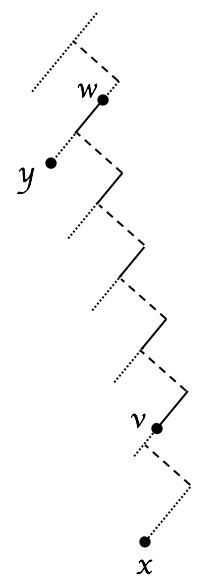
\includegraphics[scale=0.5]{rmq}
                \centering
                \caption{Demonstration of an $rmqInc$ query}
                \label{fig:rmq}
            \end{figure}

            Now, as before, we partition the path from $v$ to $w$ into a concatenation of subpaths of centroid paths, denoted by $Q_1, Q_2, ..., Q_g$. This is illustrated in Figure~\ref{fig:rmq}. This figure shows part of a tree on which an $rmqInc(v, w)$ query has been made. The diagonal lines from right to left are centroid paths in the tree (elements of $P$). The dashed edges indicate that the child is not the heaviest child of its parent, hence starting a new centroid path. The bold lines are the subpaths of centroid paths that lie on the path from $v$ to $w$. $Q_1$ is the bold centroid subpath starting from $v$ and continuing upwards till the root of that path. Similarly, $Q_g$ is the bold centroid subpath starting and $w$ and continuing downwards until the path splits from that centroid path. $Q_2$ to $Q_{g - 1}$ are the bold centroid subpaths between $Q_1$ and $Q_g$. The significance of the leaves $x$ and $y$ is explained below.

            Take any $x \in \leafset(v)$. Then $Q_2, ..., Q_{g - 1}$ are contained fully in the centroid subpaths on the path from $x$ to the root of $T$. $Q_1$ must be a subpath that starts at $v$ in some centroid path $\in P$ and ends at the root of that centroid path. $Q_g$ is a subpath that starts at some node in some centroid path $\in P$ and ends at $w$, within the same path. We address each of these three divisions separately.

            To find the maximum weight within $Q_1$, we obtain the depth of $v$ within $Q_1$ by subtracting the depth of the root of $Q_1$ from the depth of $v$. Then the maximum weight can be retrieved by querying the linear RMQ structure for this centroid path, from the root to $v$.

            To find the maximum weight for the subpaths $Q_2, ..., Q_{g - 1}$, we obtain the indices of $Q_2$ and $Q_{g-1}$ in $W_x$ using the depths of the centroid paths containing $Q_1$ and $Q_g$ respectively. The maximum weight can then be found by querying $W_x$.

            Finally, we need to find the maximum weight within $Q_g$. Observe that the key here is finding which node is at the end of $Q_g$. Let $P_i$ be the centroid path of which $Q_g$ is a subpath. Then the previous question is equivalent to finding which node in $P_i$ has $v$ in one of its side trees. Let $y$ be the leaf at the bottom of $P_i$. Then the desired node is simply $lca(y, v)$. The maximum weight within $Q_g$ can now be easily found by querying the linear RMQ structure for $P_i$, from $w$ to $lca(y, v)$.

            The decomposition step, along with computation of depths for nodes and for centroid paths can be done in $O(n)$ passes through $T$. By Lemma~\ref{lem:lca}, preprocessing $T$ for $lca$ queries takes $O(n)$ time. Storing the centroid paths in linear RMQ structures takes $O(n)$ time total, by Lemma~\ref{lem:linearrmq} and since the total size of the centroid paths is $O(n)$. By the standard argument of heavy-path decomposition, it can be seen that for each leaf, the number of centroid subpaths on the path from the leaf to the root of $T$ is $O(log\,n)$. Since there are $n$ leaves, the total time taken to construct the linear RMQ structures for each leaf is $O(n\,log\,n)$. Thus we need $O(n\,log\,n)$ preprocessing time. Further, all operations done during the query are constant time, thus the query as a whole costs $O(1)$ time.
        \end{proof}
    \end{rmqinc}

    \subsection{Answering $rmq^T(v, w)$}

    \begin{rmqstructure}
        \label{theorem:rmqstructure}
        Given a tree $T$ and nodes $v, w \in V(T)$, where $w$ is a proper ancestor of $v$, the query $rmq(v, w) = max_{u \in path(v, w)}\Omega(u)$ can be answered in $O(1)$ time with $O(n\,log\,n)$ preprocessing time.

        \begin{proof}
            $rmq(v, w) = rmqInc(v, cFD(v, w))$. By Lemmas~\ref{lem:cfd} and~\ref{lem:rmqinc}, the subqueries can be answered in constant time, given $O(n\,log\,n)$ preprocessing time.
        \end{proof}
    \end{rmqstructure}

    \section{Constructing the FDCT}
    \label{sec:freqdiffconstruction}

    Let $k$ be the number of input trees and $n$ be the size of their leafsets. We present an $O(kn\,log\,n)$ solution for the weighting step in Subsection~\ref{subsec:weighting} and an $O(n\,log\,n)$ solution for \texttt{Filter\_Clusters} in Subsection~\ref{subsec:filterclusters}, which taken together with Corollary~\ref{cor:freqdiffruntimecomponents}, allow us to construct the FDCT of $\mathcal{S}$ in $O(kn\,log\,n)$ time.

    \subsection{Weighting}
    \label{subsec:weighting}

    Given the set of trees $\mathcal{S} = \{T_1, T_2, ..., T_k\}$, where $\leafset(T_1) = \leafset(T_2) = ... = \leafset(T_k) = L$ and $n = |L|$, the weighting step computes $\Omega(u)$ for every node $u \in \bigcup_{T \in \mathcal{S}}V(T)$. Recall that $\Omega(u)$ gives the frequency of $\leafset(u)$ in $\mathcal{S}$. We divide this work (as in \cite{gawrychowski2017faster}) into the labelling and counting steps. The labelling step assigns a label to each node $u \in T, T \in \mathcal{S}$, denoted by $id(u)$, such that $id(u) \in [1 ... 2kn]$ and for any node $u' \in T', T' \in \mathcal{S}$, $id(u) = id(u')$ iff $\leafset^T(u) = \leafset^{T'}(u')$. That is, two nodes have the same label iff they are associated with the same cluster. The counting step sorts these labels, allowing us to count how many nodes exist with each label, giving us the frequencies (or the weights) of the nodes.

    Recall that the approach in \cite{gawrychowski2017faster} costs $O(kn\,log^2n)$ time. We develop a way to achieve $O(kn\,log\,n)$ time.

    First, for any tree $T$ and any cluster $C \subseteq \leafset(T)$, define $T|C$, read as ``$T$ restricted to $C$'', as the tree $T'$ with $V(T') = \{lca^T(u, v) : u, v \in C\}$ which obeys $lca^T(C') = lca^{T'}(C')$ for all $C' \subseteq C$. Intuitively, $T'$ has the leaf set $C$ and consists of all nodes in $T$ that are $lca$'s of the leaves in $C$, with these nodes connected such that they have the same ancestor/descendant relationships as they had in $T$. Figure~\ref{fig:labelclusters} demonstrates this process; the tree $T_1|L'$ is $T_1$ restricted to the cluster $\{a, b, c, d\}$. Notice how nodes that are not lcas of these leaves are removed, but the structure of the tree in relation to these leaves remains the same. Further, for any node $u$ in $T$, define the node that $u$ is associated with when $T$ is restricted to $C$ to be the shallowest descendant of $u$ that is in $T|C$, denoted as $assoc^{C}(u)$. If no such node exists, i.e. if $\leafset(u) \cap C = \emptyset$, then define for convenience a special node with an empty leaf set and id $0$ and let this be $assoc^{C}(u)$. We refer to Figure~\ref{fig:labelclusters} to show examples of this concept. Let $u$ and $v$ be the nodes in $T_1$ labelled $5, 1$ and $5, 0$ respectively. Then $assoc^{\{a, b, c, d\}}(u) = v$, since this is its shallowest descendant in $T_1|\{a, b, c, d\}$. $assoc^{\{e, f, g, h\}}(v)$ is the special node, since no descendant of $v$ is in $T_1|\{e, f, g, h\}$.

    The algorithm \texttt{Label\_Clusters} is laid out below.

    \begin{algorithm}
        \caption{Label\_Clusters}
        \label{alg:labelclusters}

        \begin{algorithmic}[1]
            \Input A set $\mathcal{S}$ of trees $\{T_1, T_2, ..., T_k\}$ where $\leafset(T_1) = \leafset(T_2) = ... = \leafset(T_k) = L$

            \Output Associate a label $id(u) \in [1 ... 2k |L|]$ with every node $u$ in the trees in $\mathcal{S}$ such that for any two nodes $v, w$ in some trees in $\mathcal{S}$, $id(v) = id(w)$ iff $\leafset(v) = \leafset(w)$.

            \State Partition $L$ into $L'$ and $L''$ such that $|L'| = |L''|$.

            \State For all $i \in [1 ... k]$, let $T'_i = T_i|L'$ and $T''_i = T_i|L''$.

            \State \texttt{Label\_Clusters}$(T'_1, T'_2, ..., T'_k)$.

            \State \texttt{Label\_Clusters}$(T''_1, T''_2, ..., T''_k)$.

            \State For every tree $T \in \mathcal{S}$, for every node $u \in T$, represent $u$ by the pair $(id(assoc^{L'}(u)), id(assoc^{L''}(u)))$.

            \State Radix sort all pairs obtained and remove duplicates. Assign a rank to each unique pair.

            \State For every tree $T \in \mathcal{S}$, for every node $u \in T$, set $id(u) = $ rank of the pair $(id(assoc^{L'}(u)), id(assoc^{L''}(u)))$.
        \end{algorithmic}
    \end{algorithm}

    One iteration of this process is illustrated in Figure~\ref{fig:labelclusters}. Here $L' = \{a, b, c, d\}$ and $L'' = \{e, f, g, h\}$. It is assumed that the algorithm has correctly labelled the clusters for each of the restricted trees, and these labels are assigned as shown. $T_1$ and $T_2$ then show the pair associated with each internal node. For example, the cluster $\{a, b, e\}$ in $T_1$ is labelled by $5$ from $\{a, b\}$ in $T_1|L'$ and $1$ from $\{e\}$ in $T_1|L''$. Similarly, the cluster $\{a, b\}$ in $T_1$ is labelled by $5$ from $\{a, b\}$ in $T_1|L'$ and $0$ from the special node since $\{a, b\} \cap \{e, f, g, h\} = \emptyset$.

    \begin{figure}[h]
        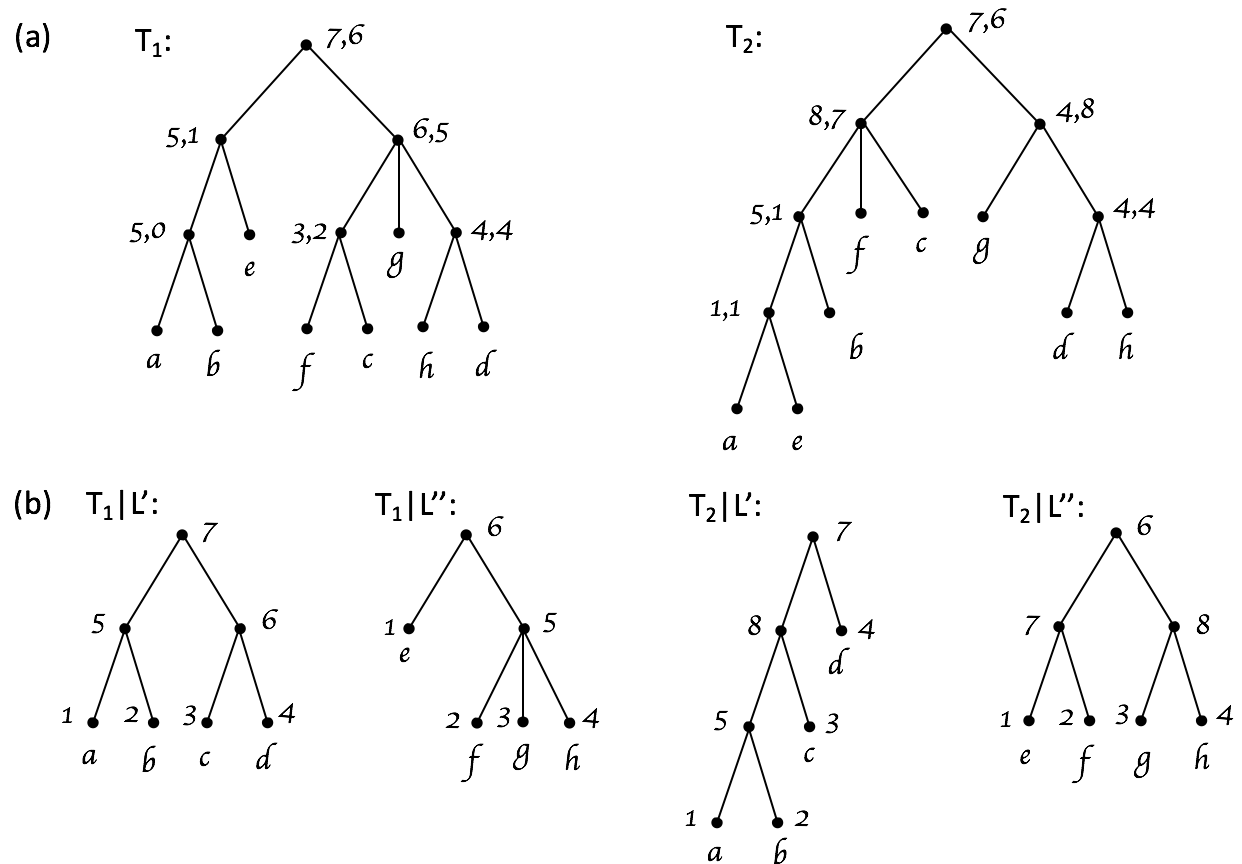
\includegraphics[scale=0.5]{labelclusters}
        \centering
        \caption{Demonstration of \texttt{Label\_Clusters}}
        \label{fig:labelclusters}
    \end{figure}

    \bigskip
    \begin{assocnode}
        \label{lem:assocnode}

        For any tree $T$, for any node $u \in V(T)$ and any cluster $C \subseteq \leafset(T)$, $\leafset^{T|C}(assoc^C(u)) = \leafset^{T}(u)\, \cap\, C$.

        \begin{proof}
            First note that for any node $v \in V(T|C)$, $\leafset^{T|C}(v) = \leafset^{T}(v)\, \cap\, C$ due to the way $T|C$ is constructed. Also, $\leafset^{T}(assoc^C(u)) \subseteq \leafset^{T}(u)$ since $assoc^C(u)$ is a descendant of $u$. Thus $\leafset^{T}(assoc^C(u))\, \cap\, C \subseteq \leafset^{T}(u)\, \cap\, C$ and so $\leafset^{T|C}(assoc^C(u)) \subseteq \leafset^{T}(u)\, \cap\, C$.

            This implies that if $\leafset^{T|C}(assoc^C(u)) \neq \leafset^{T}(u)\, \cap\, C$ then there is some leaf $x$ such that $x \in \leafset^{T}(u)\, \cap\, C$ and $x \not\in \leafset^{T|C}(assoc^C(u))$. Now, since $\leafset^{T|C}(assoc^C(u)) \subseteq \leafset^{T}(u)$ and $x \in \leafset^{T}(u)$, $\leafset^{T|C}(assoc^C(u)) \cup \{x\} \subseteq \leafset^{T}(u)$. Let $v = lca^T(\leafset^{T|C}(assoc^C(u)) \cup \{x\})$. Then $v$ is a descendant of $u$. Also, $v$ is a proper ancestor of $assoc^C(u)$. Finally, $v \in V(T|C)$. But then some ancestor of $v$ would be $assoc^C(u)$, and not the node that was initially obtained.
        \end{proof}
    \end{assocnode}

    \medskip
    \begin{labelclusterscorrectness}
        \label{lem:labelclusterscorrectness}

        After running \texttt{Label\_Clusters}$(\mathcal{S})$, for any trees $T_i, T_j \in \mathcal{S}$, for any nodes $u \in V(T_i), v \in V(T_j)$, $id(u) = id(v)$ iff $\leafset^{T_i}(u) = \leafset^{T_j}(v)$.

        \begin{proof}
            $id(u) = id(v)$ iff $id(assoc^{L'}(u)) = id(assoc^{L'}(v))$ and $id(assoc^{L''}(u)) = id(assoc^{L''}(v))$. Inductively, $id(assoc^{L'}(u)) = id(assoc^{L'}(v))$ iff $\leafset^{T_i|L'}(assoc^{L'}(u)) = \leafset^{T_j|L'}(assoc^{L'}(v))$. By Lemma~\ref{lem:assocnode}, $\leafset^{T_i}(u)\, \cap\, L' = \leafset^{T_j}(v)\, \cap\, L'$. Symmetrically, $id(assoc^{L''}(u)) = id(assoc^{L''}(v))$ iff $\leafset^{T_i}(u)\, \cap\, L'' = \leafset^{T_j}(v)\, \cap\, L''$. Since $L'$ and $L''$ partition $L$, both parts are true iff $\leafset^{T_i}(u) = \leafset^{T_j}(v)$.
        \end{proof}
    \end{labelclusterscorrectness}

    \medskip
    \begin{labelclustersidbounds}
        \label{lem:labelclustersidbounds}

        After running \texttt{Label\_Clusters}$(\mathcal{S})$, for any node $u \in V(T), T \in \mathcal{S}$, $id(u) \in [1 ... 2k |L|]$.

        \begin{proof}
            It is easily seen that $|V(T)| < 2|L|$. Thus the total number of pairs is less than $2k|L|$. This also places an upper bound on the number of ids. Notice that $u$ cannot be labelled with $0$ since that is reserved for the special node.
        \end{proof}
    \end{labelclustersidbounds}

    \medskip
    \begin{labelclustersruntime}
        \label{lem:labelclustersruntime}

        The algorithm \texttt{Label\_Clusters}$(\mathcal{S})$ runs in $O(kn\,log\,n)$ time.

        \begin{proof}
            Let $T(m)$ be the runtime of \texttt{Label\_Clusters}$(\mathcal{T})$, where $m =$ size of leaf set of each tree in $\mathcal{T}$. By Lemma 5.2 of \cite{farach1995fast}, construction of $T'_i$ and $T''_i$ takes $O(m)$ time for each $T_i \in \mathcal{T}$, taking total $O(km)$ time over all the trees. Computing $assoc^{L'}(u)$ and $assoc^{L''}(u)$ for each node $u$ in some tree $T_i \in \mathcal{T}$ can be done by a bottom up traversal of $T_i$ along with $T'_i$ and $T''_i$, taking $O(km)$ time total. Also observe that the number of pairs obtained is $O(km)$. Further, each of the values in the pair is in the range [0, km]. Thus radix sorting these pairs and assigning labels back to the nodes takes $O(km)$ time. So $T(m) = 2T(m/2) + O(km)$, giving $T(n) = kn\,log\,n$.
        \end{proof}
    \end{labelclustersruntime}

    \medskip
    \begin{weightingruntime}
        \label{lem:weightingruntime}

        The weighting step can be completed in $O(kn\,log\,n)$ time.

        \begin{proof}
            As shown in Lemma~\ref{lem:labelclustersruntime}, assigning labels to each node takes $O(kn\,log\,n)$ time. Next, we counting sort these labels. Since each label is in the range $[1 ... 2kn]$ and there are $O(kn)$ labels, this takes $O(kn)$ time. The frequencies, or weights, can then be computed in $O(kn)$ time.
        \end{proof}
    \end{weightingruntime}

    \subsection{\texttt{Filter\_Clusters}}
    \label{subsec:filterclusters}

    Given the trees $T_A$ and $T_B$ where $\leafset(T_A) = \leafset(T_B) = L$ and $n = |L|$, the algorithm \texttt{Filter\_Clusters} constructs the tree $T$ such that $\mathcal{C}(T) = \{C : C \in \mathcal{C}(T_A) \text{ and } \Omega(C) > max(\{\Omega(C_1) : C_1 \in \mathcal{C}(T_B) \text{ and } C_1 \not\compatible C\})\}$ and $\leafset(T) = L$. Recall that the previous best known solution, as in \cite{jansson2018algorithms}, costs $O(kn\,log^2n)$ time; we present an $O(kn\,log\,n)$ solution.

    The key here is finding, for any node $u \in V(T_A)$, the set of nodes in $T_B$ that are incompatible with $u$, so that we can find the maximum weight of these. Then it is easy to figure out whether $u$ should be in $T$ or not. Before describing how these nodes are found, we prove some important lemmas.
    \newline

    \begin{filterclusterssubsetcompatible}
        \label{lem:filterclusterssubsetcompatible}

        Let nodes $u \in V(T_A)$, $v \in V(T_B)$ such that $\leafset(v) \subseteq \leafset(u)$. Then for any $u' \in V(T_A) - V(T_A[u])$, and any $v' \in V(T_B[v])$, $\leafset(u') \compatible \leafset(v')$.

        \begin{proof}
            Note that $\leafset(v') \subseteq \leafset(v)$ since $v'$ is in the subtree rooted at $v$. There are two cases for $u'$. \textit{Case 1}: $u'$ is an ancestor of $u$. Then $\leafset(u) \subseteq \leafset(u')$. Thus $\leafset(v') \subseteq \leafset(u')$, and so $\leafset(v') \compatible \leafset(u')$. \textit{Case 2}: $u'$ is not an ancestor of $u$. Since $u'$ is also not a descendant of $u$, $\leafset(u') \cap \leafset(u) = \emptyset$. Thus $\leafset(u') \cap \leafset(v') = \emptyset$ and so $\leafset(v') \compatible \leafset(u')$.
        \end{proof}
    \end{filterclusterssubsetcompatible}

    The above lemma says that if $\leafset(v) \subseteq \leafset(u)$ for some nodes $v \in V(T_B)$ and $u \in V(T_A)$, then $v$ is the root of a subtree of $T_B$ that is compatible with every node in $V(T_A) - V(T_A[u])$. The upshot of this is that once we process $T_A[u]$, then for the remaining nodes in $T_A$, no node in $V(T_B[v])$ needs to be considered for incompatibility again.

    This idea is formalized as follows. For any cluster $C \subseteq L$, define any node $r \in V(T_B)$ to be the root of a \textit{maximal subtree compatible with $C$} if it satisfies the following property: $\leafset(r) \subseteq C$ and there is no proper ancestor $r'$ of $r$ such that $\leafset(r') \subseteq C$. The set $RST(C)$ is composed of all nodes $r \in V(T_B)$ that are roots of maximal subtrees compatible with $C$. Extending this, for any $u \in V(T_A)$, we denote $RST(\leafset(u))$ as $RST(u)$. For example, let $C = \{a, b, c, f, g, h\}$. Then in the tree in Figure~\ref{fig:rootsofsubtrees}, the circled nodes are the ones in $RST(C)$.

    We now prove a stronger version of Lemma~\ref{lem:incompatibility} that takes these maximal compatible subtrees into account to compute the set $incompatible(u) = \{v : v \in V(T_B) \text{ and } \leafset(v) \not\compatible \leafset(u)\}$ for any $u \in V(T_A)$.
    \newline

    \begin{incompatibilityrootsofsubtrees}
        \label{lem:incompatibilityrootsofsubtrees}

        For any node $u \in V(T_A)$, define $l_u = lca^{T_B}(\leafset(u))$. Then for any $u \in V(T_A)$, $v \in incompatible(u)$ iff $v$ is a proper descendant of $l_u$ and for some $r \in RST(u)$, $v$ is a proper ancestor of $r$, i.e. $incompatible(u) = \bigcup_{r \in RST(u)} path^{T_B}(parent(r), l_u)$.

        \begin{proof}
            $\longrightarrow$. Given some $v \in V(T_B)$ such that $\leafset(v) \not\compatible \leafset(T_A[u])$, $v$ must be a proper descendant of $l_u$ by Lemma~\ref{lem:incompatibility}. Further, for some $x \in \leafset(u)$, $v$ is a proper ancestor of $x$ by Lemma~\ref{lem:incompatibility}. Then there must be some $r \in RST(u)$ such that $r$ is an ancestor of $x$. $v \not\in V(T_B[r])$, otherwise $\leafset(v) \subseteq \leafset(u)$. Thus $v$ is a proper ancestor of $r$.

            $\longleftarrow$. Given some $v \in V(T_B)$ such that $v$ is a proper descendant of $l_u$ and for some $r \in RST(u)$, $v$ is a proper ancestor of $r$. Since $v$ is a proper descendant of $l_u$, $\leafset(u) \not\subseteq \leafset(v)$. Since $v$ is a proper ancestor of $r$, $\leafset(r) \subset \leafset(v)$, so $\leafset(v) \cap \leafset(u) \neq \emptyset$. Finally, $\leafset(v) \not\subseteq \leafset(u)$, otherwise $r \not\in RST(u)$.
        \end{proof}
    \end{incompatibilityrootsofsubtrees}

    This is illustrated in Figure~\ref{fig:rootsofsubtrees}. Here, any node in $RST(\{a, b, c, f, g, h\})$ is circled and any node that is incompatible with this cluster has a square around it. The node $l_u = lca(\{a, b, c, f, g, h\})$. As can be seen, all nodes on the path from roots of maximal subtrees to $l_u$ are incompatible with the given cluster.

    \begin{figure}[h]
        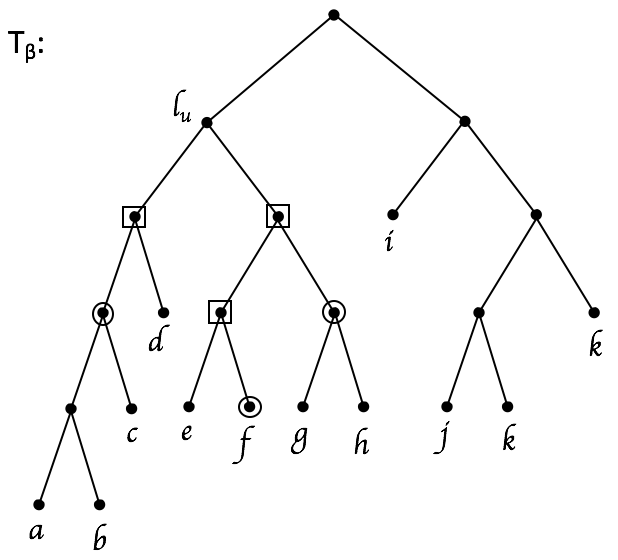
\includegraphics[scale=0.5]{rootsofsubtrees}
        \centering
        \caption{Illustration of Lemma~\ref{lem:incompatibilityrootsofsubtrees}}
        \label{fig:rootsofsubtrees}
    \end{figure}

    We now build, for any internal node $u \in V(T_A)$, a recursive definition of $incompatible(u)$, in terms of $incompatible(c_1)$, where $c_1 \in children(u)$.
    \newline

    \begin{incompatibilityrecursive}
        \label{lem:incompatibilityrecursive}

        Given any internal node $u \in V(T_A)$ and $c_1 \in children(u)$, define
        \begin{align*}
            newRST(u, c_1) &= RST(u) - RST(c_1)\\[0.5em]
            removedRST(u, c_1) &= RST(c_1) - RST(u)\\[0.5em]
            oldRST(u, c_1) &= RST(u) \cap RST(c_1)
        \end{align*}
        Then for any $r_1 \in oldRST(u, c_1)$ (if this does not exist then the relevant term below is empty),
        \begin{align*}
            incompatible(u) = &\left(incompatible(c_1)\ -\ \bigcup_{r \in removedRST(u, c_1)} path^{T_B}(parent(r), l_{c_1})\right)\\
            &\cup\ \bigcup_{r \in newRST(u, c_1)} path^{T_B}(parent(r), l_u)\\
            &\cup\ path^{T_B}(parent(r_1), l_u)
        \end{align*}

        \begin{proof}
            The intuition behind this is to see that nodes that are proper ancestors of any $r \in removedRST(u, c_1)$ and descendants of any $r' \in newRST(u, c_1)$ need to be removed from $incompatible(c_1)$ since they are compatible with $u$. This accounts for the first two lines in the statement. The last line is to ensure that nodes between $l_{c_1}$ and $l_u$ are added to the set of incompatible nodes if necessary.

            Figure~\ref{fig:incompatibilityrecursive} provides a visual illustration of this claim, showing the nodes in $T_B$ incompatible with some $u \in V(T_B)$. Here $RST(u) = \{r_1, r_3, r_4, r_5\}$ and $RST(c_1) = \{r_1, r_2\}$. The triangles under each of these nodes represent the subtrees rooted at them. The nodes on the dotted line between $r_1$ and $l_{c_1}$ are in $incompatible(c_1)$ and remain in $incompatible(u)$. The nodes on the dashed line between $r_2$ and $r_4$ are now known to be compatible with $u$, so they will be removed from $incompatible(c_1)$. The nodes on the bold lines from $r_3$, $r_4$ and $r_5$ are added to $incompatible(c_1)$ to get $incompatible(u)$. Notice that the nodes between $l_{c_1}$ and $l_u$ are added due to $r_3$ and $r_4$, but even if no root of a maximal subtree compatible with $\leafset(u)$ is in $V(T_B[l_{c_1}])$, these nodes would have been added due to $r_1$, which belongs to $oldRST(u, c_1)$.

            \begin{figure}[h]
                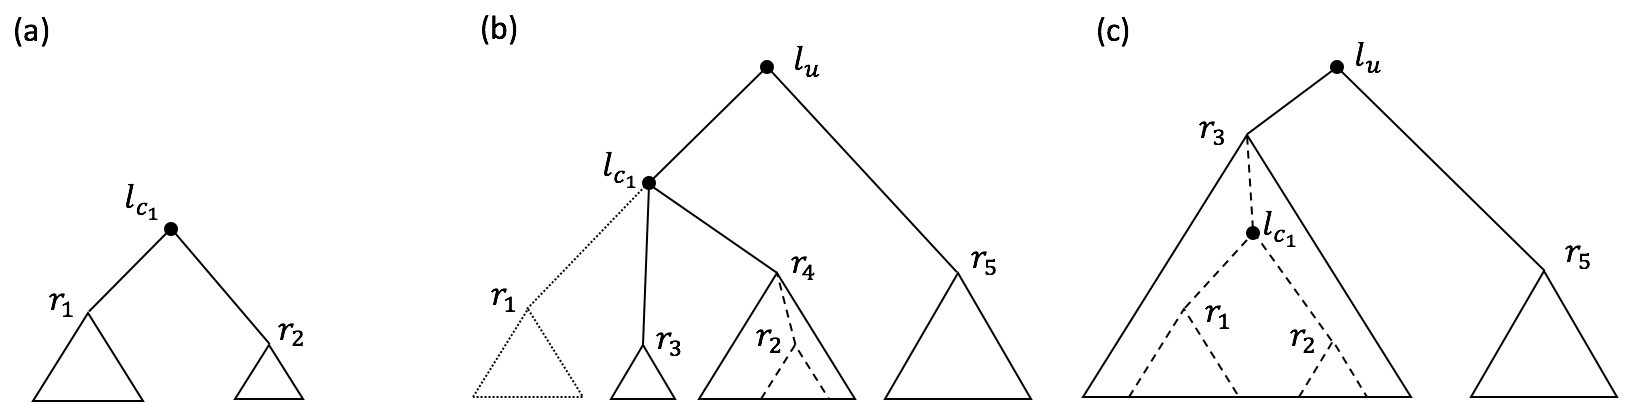
\includegraphics[scale=0.5]{incompatibilityrecursive}
                \centering
                \caption{Illustration of Lemma~\ref{lem:incompatibilityrecursive}}
                \label{fig:incompatibilityrecursive}
            \end{figure}

            We now provide a formal proof of the above claim. First, it must be true that for any $r \in removedRST(u, c_1)$, there is some $r' \in newRST(u, c_1)$ such that $r'$ is a proper ancestor of $r$. If not, then since $\leafset(r) \subseteq \leafset(c_1) \subseteq \leafset(u)$ and there is no proper ancestor $r''$ of $r$ such that $\leafset(r'') \subseteq \leafset(u)$, $r \in RST(u)$. But then $r \not\in removedRST(u, c_1)$.

            $\longrightarrow$. Let $v \in incompatible(u)$. Then by Lemma~\ref{lem:incompatibilityrootsofsubtrees}, $v$ is a proper descendant of $l_u$. If there is some $r \in newRST(u, c_1)$ such that $v$ is a proper ancestor of $r$ then $v \in path(parent(r), l_u)$. Otherwise, by Lemma~\ref{lem:incompatibilityrootsofsubtrees}, there must be some $r \in oldRST(u, c_1)$ such that $v$ is a proper ancestor of $r$. Then for all $r' \in removedRST(u, c_1)$, it cannot be that $v$ is a proper ancestor of $r'$. To see why, assume this is not true, i.e. there is some $r' \in removedRST(u, c_1)$ such that $v$ is a proper ancestor of $r'$. Then there is some $r'' \in newRST(u, c_1)$ such that $r''$ is a proper ancestor of $r'$. If $v$ is a descendant of $r''$, then $\leafset(v) \subseteq \leafset(r'') \subseteq \leafset(u)$. But then $v \not\in incompatible(u)$. Otherwise, if $v$ is a proper ancestor of $r''$, then there is some $r'' \in newRST(u, c_1)$ such that $v$ is a proper ancestor of $r''$, which contradicts our earlier assumption. Thus, if $v$ is a proper descendant of $l_{c_1}$, then $v \in incompatible(c_1)\ -\ \bigcup_{r \in removedRST(u, c_1)} path^{T_B}(parent(r), l_{c_1})$. Otherwise, for any $r_1 \in oldRST(u, c_1)$, $v \in path^{T_B}(parent(r_1), l_u)$ since $path^{T_B}(l_{c_1}, l_u) \subseteq path^{T_B}(parent(r_1), l_u)$.

            $\longleftarrow$. Let $v \in RHS$ of equation above.

            \textit{Case 1.} $v \in \bigcup_{r \in newRST(u, c_1)} path^{T_B}(parent(r), l_u)$. Then by Lemma~\ref{lem:incompatibilityrootsofsubtrees}, $v \in incompatible(u)$.

            \textit{Case 2.} $v \in path^{T_B}(parent(r_1), l_u)$. Since $r_1 \in RST(u)$, by Lemma~\ref{lem:incompatibilityrootsofsubtrees}, $v \in incompatible(u)$.

            \textit{Case 3.} $v \in incompatible(c_1)\ -\ \bigcup_{r \in removedRST(u, c_1)} path^{T_B}(parent(r), l_{c_1})$ and\\[0.25em] % Overflows otherwise
            $v \not\in \bigcup_{r \in newRST(u, c_1)} path^{T_B}(parent(r), l_u)$.\\[0.25em]
            Since $v \in incompatible(c_1)$, it is easy to see that $\leafset(v) \cap \leafset(u) \neq \emptyset$ and $\leafset(u) \not\subseteq \leafset(v)$. Also, there is some leaf $x \in \leafset(v)$ such that $x \not\in \leafset(c_1)$. If $x \in \leafset(u)$, then there is some $r \in RST(u)$ such that $r$ is an ancestor of $x$. Then $r \in newRST(u, c_1)$ since $x \in \leafset(r)$ and $x \not\in \leafset(c_1)$. We also note that $v$ is an ancestor of $x$. If $v$ is a proper ancestor of $r$, then $v \in path^{T_B}(parent(r), l_u)$, which contradicts the definition of $v$. Thus $v$ is a descendant of $r$. Since $v \in incompatible(c_1)$, there is some $r' \in RST(c_1)$ such that $v$ is a proper ancestor of $r'$ (by Lemma 10). Then $r$ is a proper ancestor of $r'$, so $r' \not\in RST(u)$. Thus $r' \in removedRST(u, c_1)$. But then $v \in \bigcup_{r \in removedRST(u, c_1)} path^{T_B}(parent(r), l_{c_1})$, which contradicts the definition of $v$. Thus $x \not\in \leafset(u)$ and so $v \in incompatible(u)$.
        \end{proof}
    \end{incompatibilityrecursive}

    We also define a property $counter(v)$ for any $v \in T_B$ (as in \cite{jansson2018algorithms}). $T_B$ satisfies the \textit{parent counter invariant} for some cluster $C \subseteq L$, denoted as $pci(C)$, iff for all nodes $v \in \bigcup_{r \in RST(C)} parent(r)$, $counter(v) = |children(v) \cap RST(C)|$.

    We thus present Algorithm~\ref{alg:computerootsofsubtrees} (on the following page) which, for some internal node $u \in V(T_A)$ and $c_1 \in children(u)$, takes in $RST(c_1)$, $LB(u, c_1) = \bigcup_{c \in children(u) - \{c_1\}} RST(c)$ and $T_B$ where $pci(\leafset(c_1]))$ holds and returns $newRST(u, c_1)$, $removedRST(u, c_1)$ and $oldRST(u, c_1)$. In addition $T_B$ is updated so that $pci(\leafset(u))$ holds.

    The algorithm iterates upwards from each node in $LB$, updating $counter$ values, and in doing so discovering which nodes are compatible with $\leafset(u)$. We prove the correctness of this algorithm below.

    \begin{algorithm}
        \caption{Compute\_Roots\_Of\_Subtrees}
        \label{alg:computerootsofsubtrees}

        \begin{algorithmic}[1]
            \Input For some internal node $u \in V(T_A)$ and $c_1 \in children(u)$, $RST(c_1)$, $LB(u, c_1)$ and $T_B$ where $pci(\leafset(c_1))$ holds with $\leafset(T_A) = \leafset(T_B) = L$.

            \Output $newRST(u, c_1)$, $removedRST(u, c_1)$ and $oldRST(u, c_1)$.

            \SideEffect $pci(\leafset(u))$ holds.

            \State $new, removed := \{\}$

            \ForAll{$v \in LB(u, c_1)$}
                \State $counter(parent(v)) := counter(parent(v)) + 1$

                \State $v := parent(v)$

                \While{$counter(v) = |children(v)|$}
                    \State $counter(parent(v)) := counter(parent(v)) + 1$

                    \State $new := (new \cup \{v\}) - children(v)$

                    \State $removed := removed \cup (children(v) \cap RST(c_1))$

                    \State $v := parent(v)$
                \EndWhile
            \EndFor

            \State $old := RST(c_1) - removed$

            \State \Return $new$, $removed$, $old$
        \end{algorithmic}
    \end{algorithm}

    \bigskip
    \begin{computerootsofsubtreescorrectness}
        \label{lem:computerootsofsubtreescorrectness}

        For any internal node $u \in V(T_A)$ and $c_1 \in children(u)$, the algorithm\\ % Overflows otherwise
        \texttt{Compute\_Roots\_Of\_Subtrees}$(RST(c_1), LB(u, c_1), T_B)$ outputs $newRST(u, c_1)$, $removedRST(u, c_1)$ and\\ % Overflows otherwise
        $oldRST(u, c_1)$.

        \begin{proof}
            We prove a loop invariant. Let the nodes in $LB$ be numbered $1$ to $\beta = |LB|$ in the order that they will be iterated over, i.e. $LB = \{r_1, r_2, ..., r_{\beta}\}$. We define $D_0 = \leafset(c_1)$ for convenience. For any $i$, $1 \leq i \leq \beta$, let $D_i = D_0 \cup \bigcup_{j = 1}^{i} \leafset(r_j)$. Define $new_i = RST(D_i) - RST(D_0)$ and $removed_i = RST(D_0) - RST(D_i)$. Then we claim that after the loop in \texttt{Compute\_Roots\_Of\_Subtrees} is finished processing $r_i \in LB$, the sets $new = new_i$ and $removed = removed_i$. Additionally, $pci(D_i)$ holds. Notice that the base case holds trivially.

            We consider the loop for $r_i \in LB$. In the following paragraphs, we demonstrate that the only nodes that need to be added or removed from $new_i$ and $removed_i$ are either proper ancestors $r_i$ or children of these nodes, hence showing that the idea of iterating upwards from $r_i$ works.

            \textit{$new_i - new_{i-1}$.} Take any $r \in new_i - new_{i-1}$. Then $r \in RST(D_i) - RST(D_{i-1}) - RST(D_0)$. Since $r \in RST(D_i) - RST(D_{i-1})$, $\leafset(r) \subseteq D_i$ and $\leafset(r) \not\subseteq D_{i-1}$. Thus there is some $x \in \leafset(r)$ such that $x \in D_i - D_{i-1}$. Note that $r$ is an ancestor of $x$. $r_i$ is also an ancestor of $x$ since $x \in D_i - D_{i-1} = \leafset(r_i)$. But $\leafset(r_i) \subseteq D_i$. Then $r$ must be an ancestor of $r_i$ since $r \in RST(D_i)$. Moreover, there can only be one such $r$, otherwise the definition of $RST(D_i)$ would be violated. As $D_i \neq D_{i-1}$, clearly $RST(D_i) - RST(D_{i-1}) - RST(D_0) \neq \emptyset$. Thus $|new_i - new_{i-1}| = 1$, where this node is the shallowest ancestor $r$ of $r_i$ for which $\leafset(r) \subseteq D_i$.

            \textit{$new_{i-1} - new_i$.} Take any $r \in new_{i-1} - new_i$. Then $r \in RST(D_{i-1}) - RST(D_i) - RST(D_0)$. If $\leafset(parent(r)) \not\subseteq D_i$ then there is some leaf $x \in \leafset(parent(r))$ such that $x \not\in D_i$. Then for any proper ancestor $r'$ of $r$, $x \in \leafset(r')$ and so $\leafset(r')) \not\subseteq D_i$. Also note that $\leafset(r) \subseteq D_{i-1} \subseteq D_i$, hence $r \in RST(D_i)$. But this contradicts the construction of $r$, hence $\leafset(parent(r)) \subseteq D_i$. Further note that the parent of $r$ must be a proper ancestor of $r_i$ since $\leafset(parent(r)) \cap (D_i - D_{i-1}) \neq \emptyset$, $\leafset(r_i) = D_i - D_{i-1}$ and $r \not\in V(T_B[r_i])$.

            \textit{$removed_i - removed_{i-1}$.} Take any $r \in removed_i - removed_{i-1}$. Then $r \in (RST(D_0) \cap RST(D_{i-1})) - RST(D_i)$. By the same argument as in the previous paragraph, the parent of $r$ must be a proper ancestor of $r_i$ such that $\leafset(parent(r)) \subseteq D_i$.

            \textit{$removed_{i-1} - removed_i$.} Take any $r \in removed_{i-1} - removed_i$. Then $r \in (RST(D_0) \cap RST(D_i)) - RST(D_{i-1})$. Since $\leafset(r) \subseteq D_0$, $\leafset(r) \subseteq D_{i-1}$. Since $r \not\in RST(D_{i-1})$, there is some proper ancestor $r'$ of $r$ such that $\leafset(r') \subseteq D_{i-1}$. But then $\leafset(r') \subseteq D_i$ and so $r \not\in RST(D_i)$. Thus $removed_{i-1} - removed_i = \emptyset$.

            The inner loop updates $new$ and $removed$ following these properties. To see this, observe that the loop is iterating upwards from $r_i$ while the node it is at has a leafset that is a subset of $D_i$. This is because if for some node $v$ it is true that $counter(v) = |children(v)|$, then for each child $v' \in children(v)$, it must be true that $\leafset(v') \subseteq D_i$ and thus $\leafset(v) \subseteq D_i$.

            We now need to show that the inner loop maintains the parent counter invariant. Note that for any $v \in V(T_B)$ that passes the while loop check, $v \not\in \bigcup_{r \in RST(D_i)} parent(r)$, so its counter is immaterial. Take the node $v$ when the loop terminates. Let the child of $v$ that was processed before this be $v'$. Then before its counter is updated in the last iteration of the loop, $counter(v) = |children(v) \cap RST(D_{i-1})|$. The only change to membership of $children(v)$ in $RST(D_i)$ is that $v'$ is also added to this set and hence the new $counter(v) := counter(v) + 1$. Also note that no other counter needs to be updated since this is the only node added to $RST(D_{i-1})$ to get $RST(D_i)$. Further, observe that the setup before the while loop ensures that the above holds even if the while loop terminates immediately, as seen by setting $v' = r_i$.

            Thus our invariants hold. Since $D_{\beta} = \leafset(u)$, the output of\\ % Overflows otherwise
            \texttt{Compute\_Roots\_Of\_Subtrees}$(RST(c_1), LB(u, c_1), T_B)$ is as expected.
        \end{proof}
    \end{computerootsofsubtreescorrectness}

    \begin{computerootsofsubtreesruntime}
        \label{lem:computerootsofsubtreesruntime}

        For any internal node $u \in V(T_A)$ and $c_1 \in children(u)$, the algorithm\\ % Overflows otherwise
        \texttt{Compute\_Roots\_Of\_Subtrees}$(RST(c_1), LB(u, c_1), T_B)$ runs in\\ % Overflows otherwise
        $O(|LB(u, c_1)| + |removedRST(u, c_1)|)$ time.

        \begin{proof}
            We implement each of the set of nodes using a linked list, while augmenting the nodes with a property that lets us know whether it belongs to the set or not. This allows us to perform operations like union, intersection and set difference in time proportional to the size of either of the sets.

            The outer loop is entered $O(|LB(u, c_1)|)$ times.

            No node is added to $removed$ twice. This is because when a node is added to $removed$, the leafset of the parent of this node is known to be a subset of $D_i$, for some $i$. Then it can never be encountered again when iterating upwards from $r_j$, $j > i$. Thus the total cost of the processing inside the inner loop is $O(|removedRST(u, c_1)|)$.

            Finally, to ensure that the last set difference happens in $O(|removedRST(u, c_1)|)$, we modify the linked list $RST(c_1)$ and return this as $oldRST(u, c_1)$.

            Thus the total time taken is $O(|LB(u, c_1)| + |removedRST(u, c_1)|)$.
        \end{proof}
    \end{computerootsofsubtreesruntime}

    We now build the solution for \texttt{Filter\_Clusters}. We define a subroutine \texttt{Filter\_Clusters\_Helper} which takes as input a subtree of $T_A$ (say $T_A[u]$) and $T_B$. It returns $RST(u)$. As a side effect, any node $u' \in V(T_A[u])$ is marked for deletion if $\Omega(u') \leq max(\{\Omega(C_1) : C_1 \in \mathcal{C}(T_B) \text{ and } C_1 \not\compatible \leafset(u')\})$. This means that any node in $T_A$ which is not more frequent that every cluster it is incompatible with in $T_B$ is marked for deletion. Then \texttt{Filter\_Clusters} uses \texttt{Filter\_Clusters\_Helper} in the following manner:

    \begin{algorithm}
        \caption{Filter\_Clusters}
        \begin{algorithmic}[1]
            \Input Trees $T_A$ and $T_B$ with $\leafset(T_A) = \leafset(T_B) = L$ where every cluster has a known $weight$.

            \Output A tree $T$ where $\mathcal{C}(T) = \{C : C \in \mathcal{C}(T_A) \text{ and } \Omega(C) > max(\{\Omega(C_1) : C_1 \in \mathcal{C}(T_B) \text{ and } C_1 \not\compatible C\})\}$ and $\leafset(T) = L$

            \State Preprocess $T_B$ for $lca$ queries

            \State Do a bottom-up traversal of $T_B$ to compute $|children(v)|$ for all $v \in V(T_B)$

            \State Construct an RMQ structure over $T_B$

            \State Let $T_{A1} :=$ copy of $T_A$

            \State \texttt{Filter\_Clusters\_Helper}$(T_{A1}, T_B)$

            \State Do a top-down traversal of $T_{A1}$, deleting all marked nodes

            \State \Return $T_{A1}$
        \end{algorithmic}
    \end{algorithm}

    \texttt{Filter\_Clusters\_Helper} decomposes $T_A$ into a \textit{centroid path} and a set of \textit{side trees} (similarly to \cite{jansson2018algorithms}). Observe that for any side tree $\tau \in \sigma(\pi)$, $|\leafset(\tau)| \leq n/2$ and that $\{\leafset(\tau) : \tau \in \sigma(\pi)\}$ forms a partition of $L\, \backslash\, {p_1}$. We further note that for any $i \geq 2$, $\leafset(p_{i - 1}) \subset \leafset(p_i)$, i.e. the cluster associated with $p_{i-1}$ is a proper subset of $p_i$. This then leads to the intuition behind \texttt{Filter\_Clusters\_Helper} - recursively run \texttt{Filter\_Clusters\_Helper} on the side trees, then for the nested clusters rooted at nodes in the centroid path, use Algorithm~\ref{alg:computerootsofsubtrees} to find the roots of maximal compatible subtrees and Lemma~\ref{lem:incompatibilityrecursive} to find incompatible nodes.

    A crucial part of this algorithm is the usage of an RMQ structure on $T_B$ that allows us to query for the maximum weight of any node on the path between two given nodes (described in Section~\ref{sec:rmqstructure}). This is because we do not actually need the set of incompatible nodes, we just need to find the largest weight over all incompatible nodes. Thus, rather than inserting all the nodes in say $path^{T_B}(v, v')$ into a set, we just insert $v$ indexed by $rmq^{T_B}(v, v')$ (as obtained from the RMQ structure) into a priority queue. Notice that this plays well with Lemma~\ref{lem:incompatibilityrecursive}, which formulates incompatible nodes solely in terms of paths.

    The algorithm initialises $roots$ with $p_1$ and sets up $T_B$ to satisfy $pci(\{p_1\})$. It then uses Algorithm~\ref{alg:computerootsofsubtrees} and Lemma~\ref{lem:incompatibilityrecursive} to find the nodes incompatible with any $p_i \in \pi$. Thus it uses $incompatible(p_{i-1})$ and $RST(c)$ for each $c \in children(p_i)\, \backslash\, p_{i-1}$ to compute $incompatible(p_i)$. To facilitate this process, \texttt{Filter\_Clusters\_Helper} returns $RST(\leafset(T_A))$ for the caller to use. Once $incompatible(p_i)$ is computed, we compare the largest weight in this set with the weight of $p_i$, and mark $p_i$ for deletion if its weight is not larger.

    Finally note that we need to erase the counter values set in a call to \texttt{Filter\_Clusters\_Helper}, otherwise they will interfere with the processing of other calls. However, observe that we do not need to erase counters of any node in a compatible subtree, since those nodes will never be encountered again. Further, due to the way the algorithm is structured, the only other counters that are set are those of the parents of these subtrees, and erasing these is done at the end of a given call to the function.

    The resulting algorithm is presented on the following page.

    \begin{algorithm}[ht]
        \caption{Filter\_Clusters\_Helper}
        \label{alg:filterclustershelper}

        \begin{algorithmic}[1]
            \Input Trees $T_A$ and $T_B$ with $\leafset(T_A) \subseteq \leafset(T_B) = L$ where every cluster has a known $weight$.

            \Output $RST(\leafset(T_A))$

            \SideEffect Marks any node $u \in V(T_A)$ for deletion iff $\Omega(u) \leq \Omega(v)$ for any $v \in V(T_B)$ with $\leafset(u) \not\compatible \leafset(v)$.

            \State Compute a centroid path $\pi = \langle p_{\alpha}, p_{\alpha - 1}, ..., p_1 \rangle$ of $T_A$, where $p_{\alpha}$ is the root of $T_A$ and $p_1$ is a leaf.

            \State \algorithmicforall\ side trees $\tau \in \sigma(\pi)$,
                associate \texttt{Filter\_Clusters\_Helper}$(\tau, T_B)$ with $\tau$

            \State Let $l_1 :=$ leaf in $T_B$ labelled by $p_1$

            \State $counter(parent(l_1)) := 1$

            \State $roots := \{l_1\}$

            \State $incompatible :=$ empty Brodal queue

            \For{$i := 2$ \textbf{to} $\alpha$}
                \State $lowerBoundary := \{\}$

                \ForAll{side trees $\tau$ associated with $p_i$}
                    \State $lowerBoundary := lowerBoundary\ \cup$ list of roots associated with $\tau$
                \EndFor

                \State $new, removed, old :=$ \texttt{Compute\_Roots\_Of\_Subtrees}$(roots, lowerBoundary, T_B)$

                \State $l_i := lca^{T_B}(l_{i-1} \cup lowerBoundary)$

                \State \algorithmicforall\ $r \in removed$, remove $r$ from $incompatible$
                \label{step:removedrootsremoval}

                \State \algorithmicforall\ $r \in new$, add $r, rmq(parent(r), l_i)$ to $incompatible$

                \If{$old \neq \emptyset$}
                    \State For any $r_1 \in old$, remove $r_1$ from $incompatible$
                    \label{step:oldrootremoval}

                    \State For the same $r_1 \in old$, add $r_1, rmq(parent(r_1), l_i)$ to $incompatible$
                \EndIf

                \IIEf{$incompatible$ is empty}
                    {$M := 0$}
                    $M :=$ maximum weight of a node in $incompatible$

                \IIf{$\Omega(p_i) \leq M$}
                    mark $p_i$ for deletion

                \State $roots := old \cup new$
            \EndFor

            \State \algorithmicforall\ $r \in roots$, $counter(parent(r)) := 0$

            \State \Return $roots$
        \end{algorithmic}
    \end{algorithm}

    \bigskip
    \begin{filterclustersruntime}
        \label{lem:filterclustersruntime}

        The algorithm \texttt{Filter\_Clusters}$(T_A, T_B)$ runs in $O(n\,log\,n)$ time.

        \begin{proof}
            We preprocess $T_B$ for \textit{lca} queries using the technique of \cite{bender2000lca}. This takes $O(n)$ preprocessing time and thereafter allows us to answer \textit{lca} queries in $O(1)$ time. $T_B$ is also preprocessed for RMQ queries using Theorem~\ref{theorem:rmqstructure}. This takes $O(n\,log\,n)$ preprocessing time and thereafter allows us to answer $rmq$ queries in $O(1)$ time. The bottom-up traversal of $T_B$ to compute $|children(v)|$ for all $v \in V(T_B)$ takes $O(n)$ time. Finally, copying $T_A$ takes $O(n)$ time.

            As before, we use linked lists to implement sets of nodes, coupled with membership properties.

            The data structure used for $incompatible$ is the Brodal queue of \cite{brodal1995fast}. This allows $insert$ and $findMax$ operations in $O(1)$ time and $delete$ in $O(log\,m)$ time (where $m$ is the number of elements in the queue). Since the number of nodes in $T_B$ is $O(n)$, the number of elements in the queue is always $O(n)$ and so deletions cost $O(log\,n)$ time.

            Let $m = |\leafset(T_A)|$ for some call to \texttt{Filter\_Clusters\_Helper}$(T_A, T_B)$. Observe that for any cluster $C$, the number of compatible subtrees that can be discovered is $O(|C|)$. Recall that $n = |\leafset(T_B)|$.

            Computing the centroid path takes $O(m)$ time. Since the total number of leaves over all side trees is $O(m)$, the additions to $lowerBoundary$ cost $O(m)$ time. The calls to \texttt{Compute\_Roots\_Of\_Subtrees} cost $O(m)$ time due to $lowerBoundary$ and $O(1)$ time for each node over all calls to \texttt{Filter\_Clusters\_Helper} (since any node belongs to $removed$ only once). Since $lca$ queries can be made in constant time and the total number of $lca$ queries is $O(m)$, this also costs $O(m)$ time. $O(m)$ insertions are made into $incompatible$, costing $O(m)$ time. Since any node belongs to $removed$ only once, there are a total of $O(n)$ deletions over all calls due to Step~\ref{step:removedrootsremoval}. Step~\ref{step:oldrootremoval} also causes a total of $O(n)$ deletions over all calls as this step happens once for each node in the centroid path, and every node in $T_A$ belongs to exactly one centroid path. Thus deletions cost a total of $O(n\,log\,n)$ time.

            We can hence write a recurrence for \texttt{Filter\_Clusters\_Helper} (ignoring steps that are being analysed over the entire call to \texttt{Filter\_Clusters}) in the following manner: $T(m) = \sum_{\tau \in \sigma(\pi)}T(|\leafset(\tau))|) + O(m)$. Since for any $\tau \in \sigma(\pi)$, $|\leafset(\tau)| \leq m/2$, there are $log\,m$ recursion levels, we get $T(n) = O(n\,log\,n)$.

            Finally, we note that time taken to process $T_{A1}$ after \texttt{Filter\_Clusters\_Helper} is done takes $O(n)$ time. This is because deleting all marked nodes can be done in a top down traversal (using the \texttt{delete} operation described in Subsection~\ref{subsec:delete}), where every node's parent changes at most once. Further, recall that the total preprocessing time is $O(n\,log\,n)$ and the time set aside to be analysed over the entire call to \texttt{Filter\_Clusters} is $O(n\,log\,n)$. Thus, \texttt{Filter\_Clusters} runs in $O(n\,log\,n)$ time.
        \end{proof}
    \end{filterclustersruntime}

    \subsection{\texttt{Frequency\_Difference}}

    \begin{freqdiffruntime}
        \label{theorem:freqdiffruntime}

        The algorithm \texttt{Frequency\_Difference} runs in $O(kn\,log\,n)$ time.

        \begin{proof}
            By Corollary~\ref{cor:freqdiffruntimecomponents} and Lemmas~\ref{lem:weightingruntime} and~\ref{lem:filterclustersruntime}, \texttt{Frequency\_Difference} runs in $O(kn\,log\,n + k \cdot n\,log\,n) = O(kn\,log\,n)$ time.
        \end{proof}
    \end{freqdiffruntime}

    \newpage
    \bibliographystyle{plain}
    \bibliography{interim_report}
\end{document}
